% !TeX spellcheck = en_US
% !TeX root = ./0_article.tex

\documentclass[lettersize,journal]{IEEEtran}
\usepackage{amsmath,amsfonts}
\usepackage{algorithmic}
\usepackage{algorithm}
\usepackage{array}
\usepackage[caption=false,font=normalsize,labelfont=sf,textfont=sf]{subfig}
\usepackage{textcomp}
\usepackage{stfloats}
\usepackage{float}
\usepackage{url}
%\usepackage{natbib}
\usepackage{verbatim}
\usepackage{graphicx}
\usepackage{cite}
\usepackage{lipsum}
\usepackage{xcolor}
\usepackage{tabularx}
\usepackage{subfloat}
\usepackage{fancybox}
\usepackage[utf8]{inputenc}

\usepackage[inline]{showlabels}
%\usepackage[final]{showlabels}

\hyphenation{op-tical net-works semi-conduc-tor IEEE-Xplore}
\def\BibTeX{{\rm B\kern-.05em{\sc i\kern-.025em b}\kern-.08em
		T\kern-.1667em\lower.7ex\hbox{E}\kern-.125emX}}
\usepackage{balance}

\begin{document}
%	\title{IEEE TCAD BBI ARTICLE (MAX 14 PAGES)}
	\title{Body biasing injection: analysis, modeling and simulation (MAX 14 PAGES)}
	\author{Geoffrey Chancel}
	\markboth{Journal of \LaTeX\ Class Files,~Vol.~3, No.~4, October~2077}%
	{Shell \MakeLowercase{\textit{et al.}}: A Sample Article Using IEEEtran.cls for IEEE Journals}
	\maketitle

	% !TeX spellcheck = en_US
% !TeX root = ./0_article.tex

\begin{abstract}
	This is the abstract.
\end{abstract}

\begin{IEEEkeywords}
	Article submission, IEEE, IEEEtran, journal, \LaTeX, paper, template, typesetting.
\end{IEEEkeywords}
	% !TeX spellcheck = en_US
% !TeX root = ./0_article.tex

\section{Introduction}
%\IEEEPARstart{S}{everal} researches have studied Body Biasing Injection (BBI) in the past few years.
%While this injection method had been \textcolor{orange}{paused/forgotten} for a few years, it has recently regained some interest.
%Among the latest studies, a modeling and simulation flow has been proposed, alongside better platforms allowing to achieve greater reproducibility and a deeper analysis of the mechanisms at works in digital integrated circuits subjected to BBI.
%In addition to that

%	\subsection{Context}
	\IEEEPARstart{N}{owadays}, electronic devices are found in every economic sector, and very often manipulate sensitive and confidential data, such as in bank transactions, Internet of Things (IoT) devices, smartcards, or smartphones.
	To ensure data authenticity and confidentiality, these devices embed cryptographic algorithms.
	While theoretically secure and robust, once implemented on actual devices, these algorithms become fallible by leaking the manipulated data through various physical quantities such as electromagnetic waves, infrared emissions, or sound emissions, not to cite them all, in addition to being sensitive to external disturbances.
	
	In this context, cybersecurity takes place, more specifically hardware security.
	When comes hardware security often comes side-channel attacks and fault injection attacks.
	On the one hand, side-channel attacks take advantage of the circuit leakage by measuring the various physical quantities available.
	On the other hand, fault injection aims at inducing physical disturbances into circuits, with methods like Electromagnetic Fault Injection (EMFI) \cite{mathieuEMFIFirst, mathieuEMFI}, Laser Fault Injection (LFI) \cite{lfiFaultModel}, or Body Biasing Injection (BBI) \cite{bbiOrigin}, not to cite them all.
	Among these methods, EMFI and LFI are widely studied and understood.
	However, despite a resurgence in the past few years, BBI knowledge is still less mature compared to the previously cited methods.
	Therefore, this article is dedicated in presenting our work on Body Biasing Injection.
	
%	\IEEEPARstart{W}{hen} working with cybersecurity, more specifically with hardware security, involving various integrated circuits ranging from smartcards, smartphones, or microcontrollers, various fault injection methods are often considered.
%	We can point out some of the most documented methods such as Electromagnetic Fault Injection (EMFI) \cite{mathieuEMFIFirst, mathieuEMFI}, Laser Fault Injection (LFI) \cite{lfiFaultModel}, or Body Biasing Injection (BBI) \cite{bbiOrigin}, not to cite them all.
%	Our work is dedicated in studying Body Biasing Injection.



	\subsection{Fault injection objectives}
		Before going further in the discussion about BBI, let us first outline the main objectives of fault injection methods.
		Most commonly, they are set up to perform various malicious manipulation on integrated circuits, such as:
		\begin{itemize}
			\item Denial of service (DoS) \textrightarrow\ Stop circuit operation and the related services;
			\item Verification bypass \textrightarrow\ Modify data on the fly to fake authenticity (e.g. to bypass bootloader security);
			\item Confidential data extraction \textrightarrow\ Modify data to perform differential fault analysis.
		\end{itemize}
		To perform these objectives, we can use various injection methods, such as EMFI, LFI or BBI.
		Before presenting our work on BBI further, let us analyze the available and existing BBI platforms in the state-of-the-art.
%		\textcolor{red}{To finish.}

	\subsection{BBI in the state-of-the-art}
	\textcolor{red}{Fait-on vraiment un paragraphe sur les plateformes industrielles comme dans la thèse ?}
		When compared to EMFI, BBI has a smaller state-of-the-art, whether in the amount of scientific papers published or in the amount of industrial platforms proposed.
		Currently, there are ten main works lingering on BBI \cite{bbiOrigin, bbiSecond, bbiThird, bbiColin,japbbi, japbbi2, mybbiCosade, mybbiFdtc2022, mybbifdtc2023, colinFdtc2023}.
		Each one of them made a unique contribution for a better understanding of BBI.

		The first one \cite{bbiOrigin} introduced the technique and presented a Bellcore attack on the targeted IC.
		Then, one year later, another work \cite{bbiSecond} further studied the method, followed by a third work three years later \cite{bbiThird}, introducing an advanced test bench to work and perform attacks with BBI.
		After that, another work presented a low-cost BBI platform, dedicated to WLCSP devices \cite{bbiColin}.

		However, there are still unanswered questions, and the current works aims at bringing more answers thanks to previous and new data.

		Before introducing the present work, let us eventually analyze the industrial platforms proposed by various manufacturers and introduce our own test platform.
		We can distinguish three major actors proposing BBI related products:
		\begin{itemize}
			\item Langer EMV-Technik;
			\item Riscure;
			\item NewAE Technology.
		\end{itemize}

		% !TeX spellcheck = en_US
% !TeX root = ./0_article.tex

\begin{figure}
	\centering
	\subfloat[][Langer]{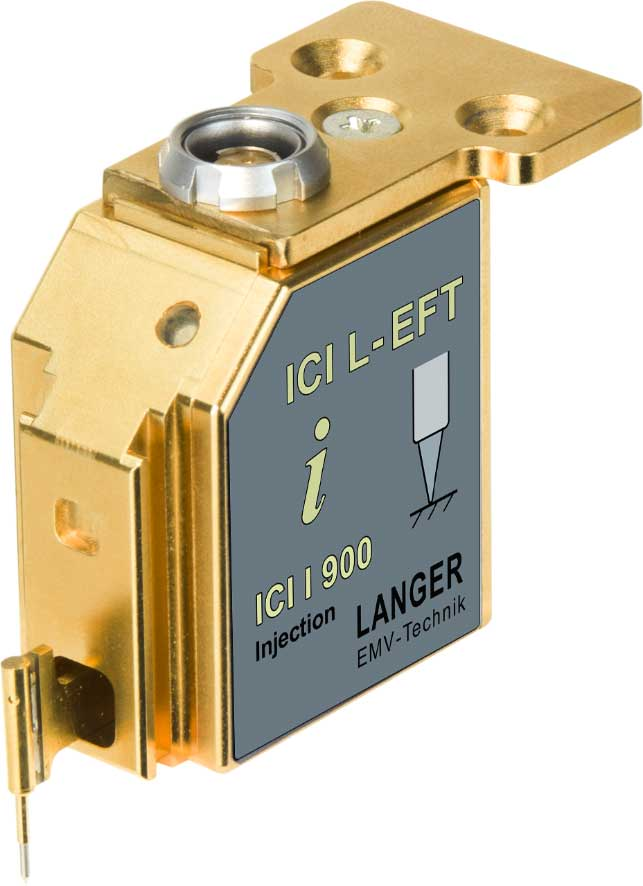
\includegraphics[width=0.2\columnwidth]{./figures/langerBBI.jpg}}
	\hspace{0.1\columnwidth}
	\subfloat[][Riscure]{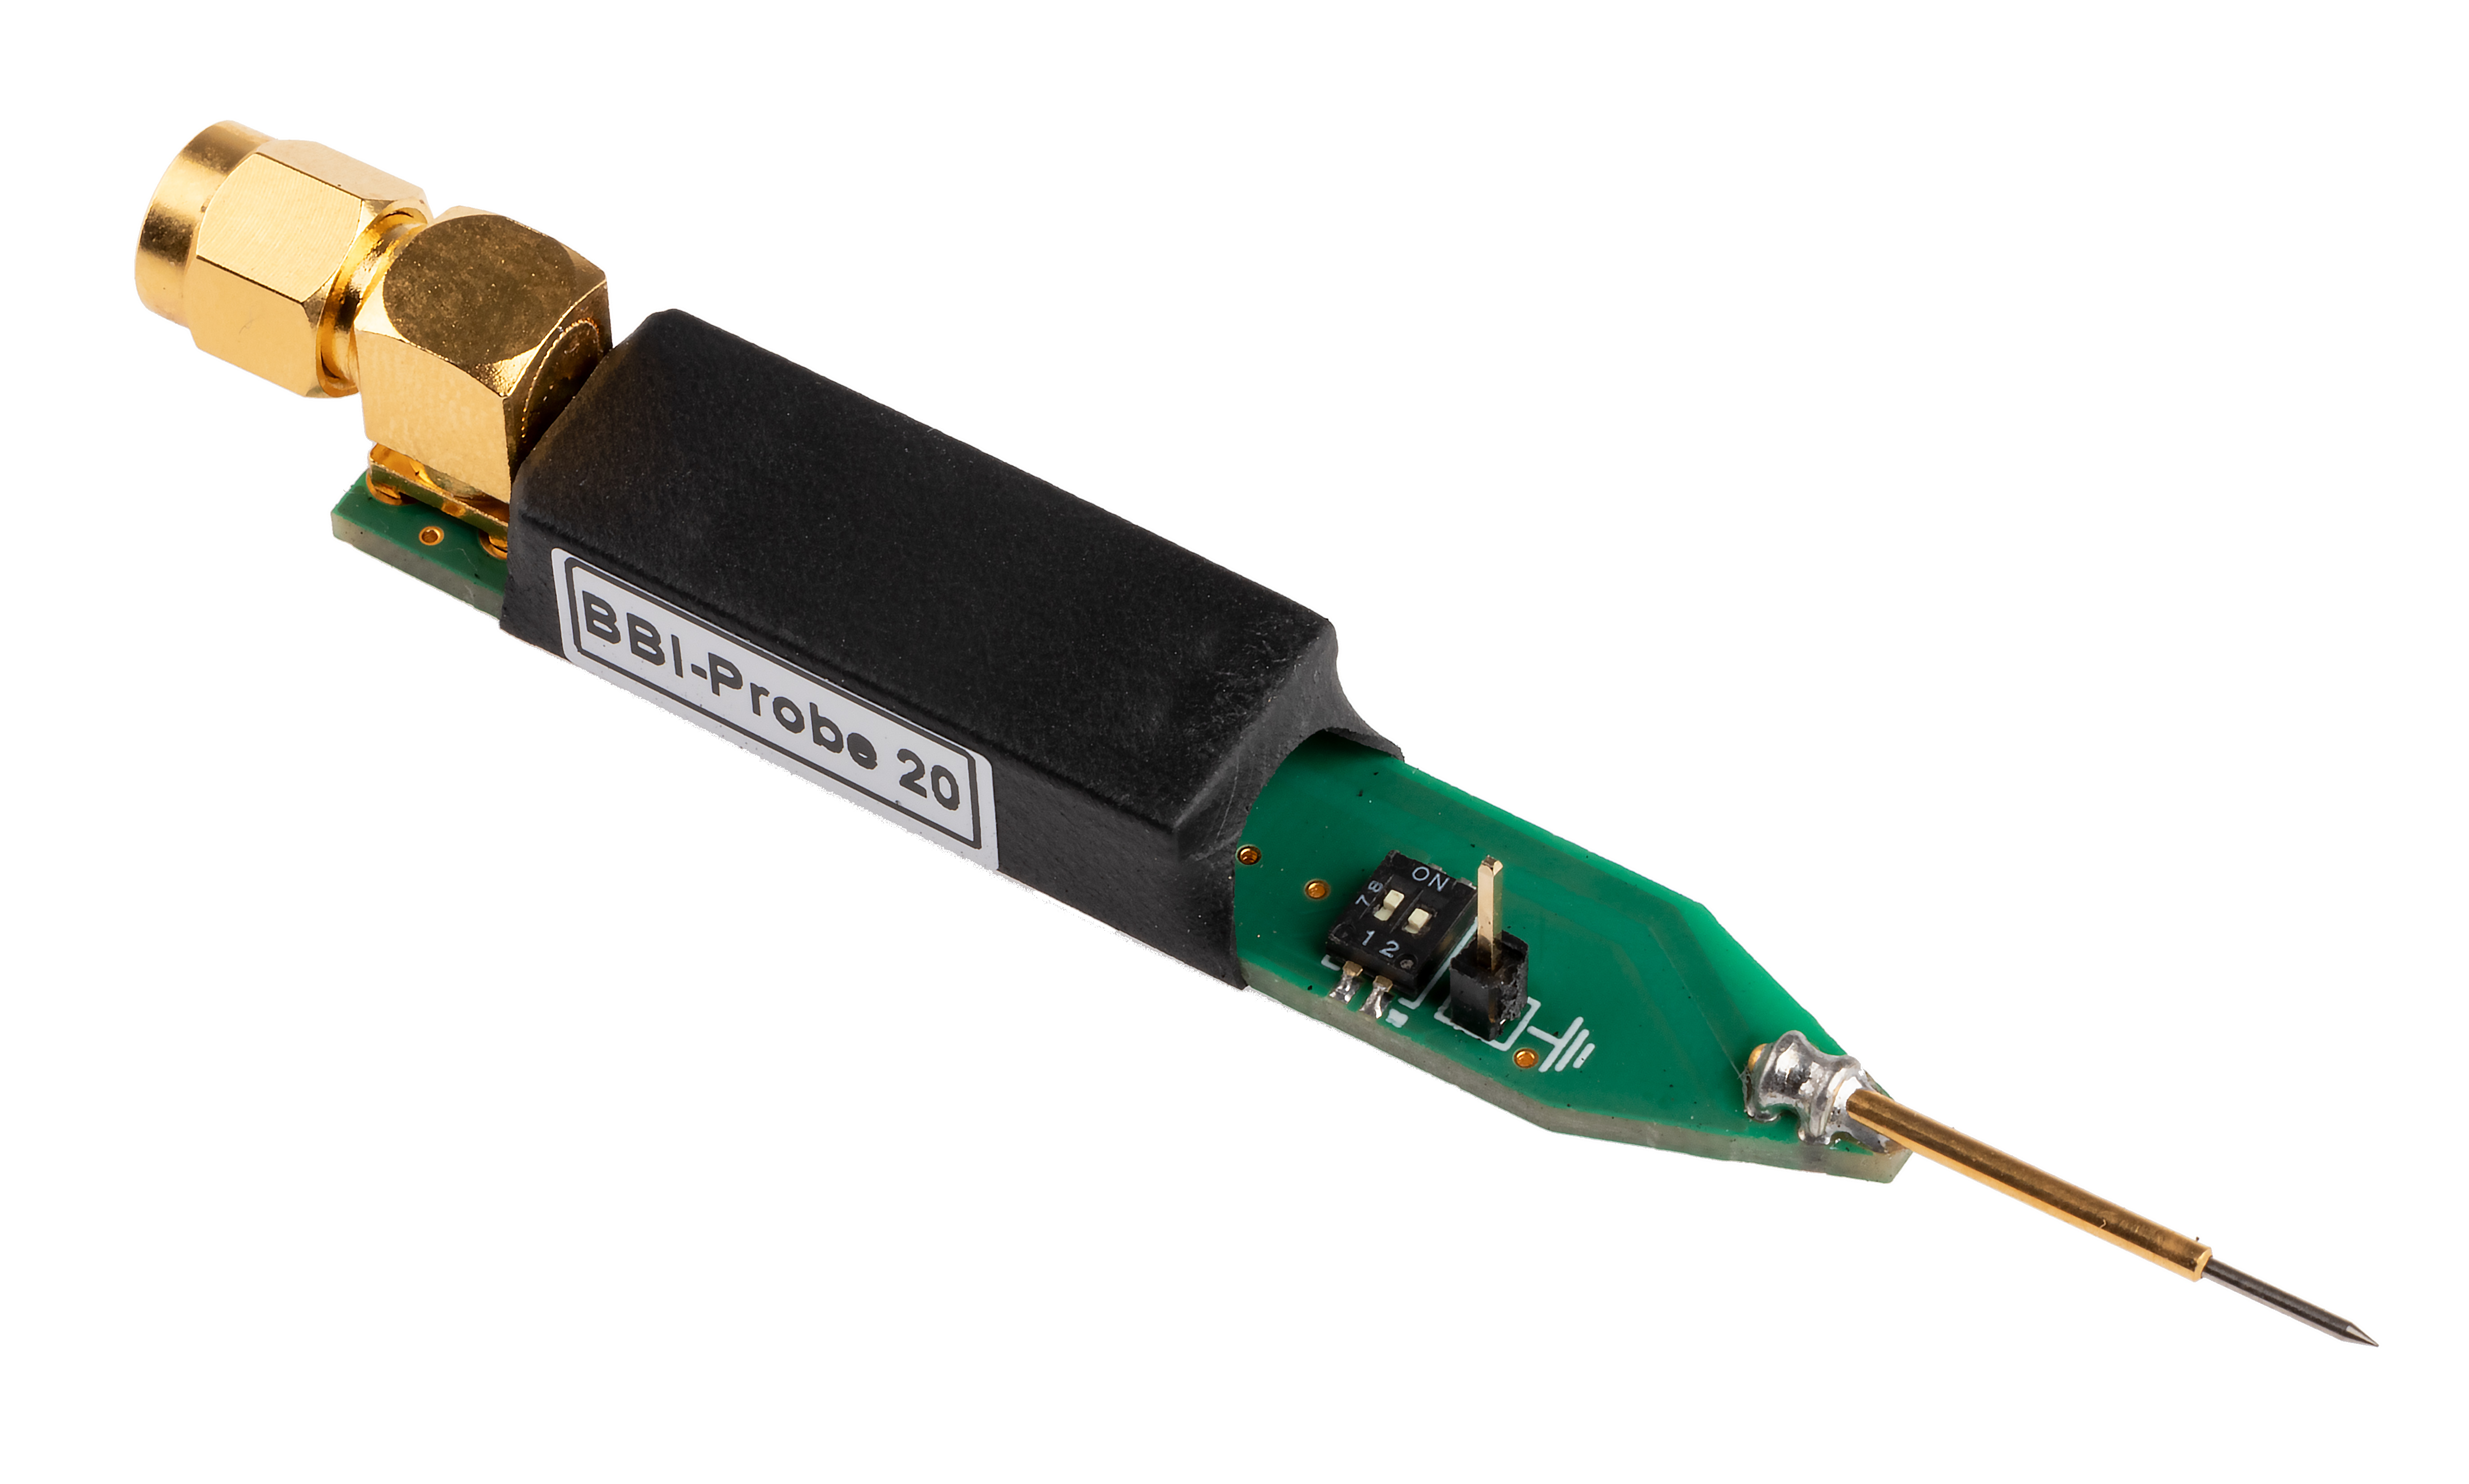
\includegraphics[width=0.425\columnwidth]{./figures/em-fi-bbi-probe-20-black.jpg}}
	\caption{Langer and Riscure BBI probes.}
	\label{riscure_langer}
\end{figure}
		\subsubsection{Langer EMV-Technik platform}
			The German society Langer EMV-Technik proposes an all-in-one and ready-to-use BBI platform composed of two hardware tools:
			\begin{itemize}
				\item A current pulse generator with a metal needle, shown in left in Fig. \ref{riscure_langer};
				\item A general controller called "Burst Power Station", combining a power supply, control and monitor tool and a software.
			\end{itemize}

	\subsection{BBI interrogations}
		With all the work in the state-of-the-art in mind, there are still remaining questions unanswered about BBI, such as:
		\begin{itemize}
			\item What is the spatial resolution of BBI?
			\item What is the time resolution of BBI?
			\item Is thinning the substrate useful in any way?
			\item How BBI induced faults occur?
			\item How to properly model BBI?
		\end{itemize}

	% !TeX spellcheck = en_US
% !TeX root = ./0_article.tex

\section{Modeling and simulating BBI}
\IEEEPARstart{S}{imulating} a fault injection method behavior is an important part in understanding its mechanisms.
Whether it is EMFI, LFI or BBI, it allows to predict and understand the underlying phenomena at work to set up reliable experiments.
In this paper, we are focusing solely on BBI.

Ideally, we would want to directly observe signals inside integrated circuits, allowing for fine measurements of power supply voltages, logic levels and power current not to cite every physical quantity.
However, embedding sensors into an already existing IC is not possible, and doing so on future IC is costly and takes time to fully implement.
In addition to this, we do not have any guarantee that these sensors will not be disturbed too much by the fault injection.
Therefore, we have decided to take the following approach:
\begin{center}
	Simulation \textrightarrow\ Conclusions \textrightarrow\ Verification
\end{center}

By doing so, we have freed ourselves from hardware limitations.
However, other limitations remains.
Indeed, modern ICs, even the smallest, embed millions of transistors, and with current technologies, it is impossible to evaluate with simulations entire circuits at a transistor level.
Therefore, to tackle these limitations, we decided to adopt an hybrid approach, combining transistor-less models and local logic gates simulations.
This approach is a compromise between accuracy and computational cost/time, and allows simulating relatively big circuits under BBI disturbances
Overall, it is similar to what has been done for EMFI in \cite{mathieuEMFI}.
The resulting simulation flow is divided in three consecutive steps:
\begin{itemize}
	\item The simulation of an IC under BBI using a transistor-less model, allowing for a purely electrical analysis;
	\item The extraction of significant disturbed signals from the previous simulation;
	\item The simulation of functional logic gates under BBI thanks to the previously extracted signals.
\end{itemize}

\subsection{An hybrid simulation flow: building the models}
	Building the correct models for the simulation flow pass through multiple steps.
	As the goal of the hybrid flow is to reduce the computational power required to evaluate an IC, it is still important to maintain a certain accuracy concerning the IC physical structure.
	To do so, the models are designed around actual IC implementations.
	The main building blocks of the models are the power supply network, the standard-cells, and the substrate structure.
	In this work, we are only focusing on bulk substrates: specifically dual-well and triple-well substrates.

	\subsubsection{Power supply rails and standard-cell segments}
		% !TeX spellcheck = en_US
% !TeX root = ./0_article.tex
% LABEL AFTER CAPTION WESH GEOFFREY !!
\begin{figure}[h]
	\centering
	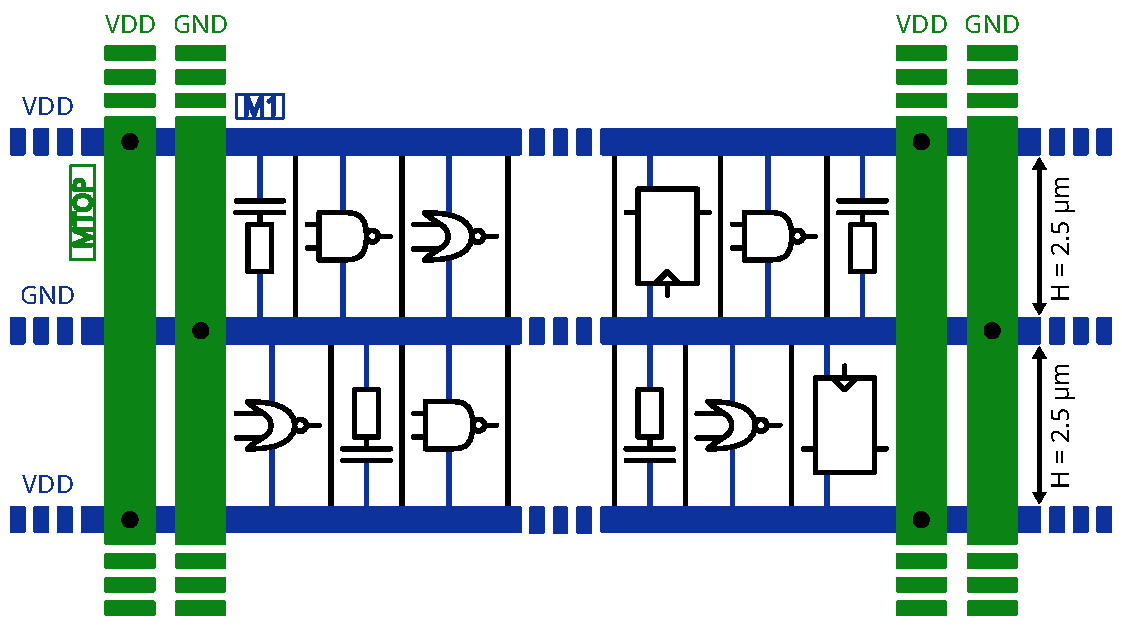
\includegraphics[width=0.49\textwidth]{./figures/psu_std_cell.pdf}
	\caption{A Standard-Cell Segment and its power delivery network.}
	\label{fig_alim_std}
\end{figure}

		The power distribution inside an IC is typically made with a grid-like structure, composed of metal wires stacked on top of each other on planes.
		In each layer, the metal wires are equally spaced and have a dedicated width, which becomes thinner the deeper they are.
		The lowest layer brings the power directly to the transistors.
		Fig. \ref{fig_alim_std} presents a common power delivery network, designed with two metal levels for simplicity.

		Within the metal lines are located standard-cell segments (SCS), composed of decoupling, logic and sequential elements, and are pre-characterized by foundries and categorized depending on their performance (mainly but not exclusively power consumption and speed).
		As illustrated in Fig. \ref{fig_alim_std}, SCS have a constant height, in our case of 2.5 \textmu m, and a variable width depending on how much logic gates each one of them embed.
		As we have stated previously, the hybrid simulation flow use transistor-less models as basic IC building blocks.
		Therefore, the transistors, hence the standard-cell segments, are modeled with passive elements such as resistors and capacitors.

		% !TeX spellcheck = en_US
% !TeX root = ./0_article.tex

\begin{figure}[h]
	\centering
	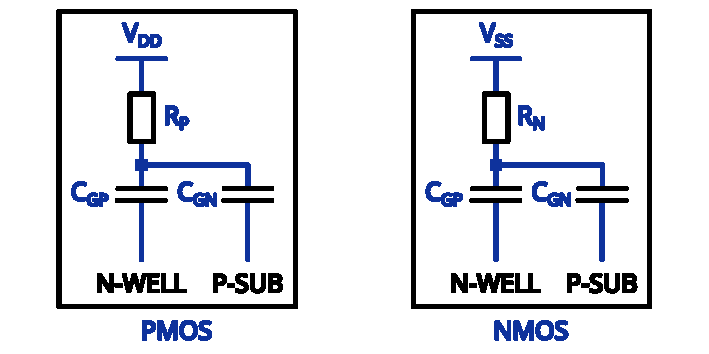
\includegraphics[width=0.9\columnwidth]{./figures/std_cell_logic_passive.pdf}
	\caption{Transistor-less equivalent model of a set of PMOS and NMOS in a SCS.}
	\label{mos_passive}
\end{figure}

		To that end, the elementary SCS chosen measures 30 \textmu m by 5 \textmu m, representing two rows of logic cells.
		This represents about a hundred of logic gates, represented with four resistors and two capacitors, as shown in Fig. \ref{mos_passive}, with half of the transistors conducting, half not conducting.
	%	Respectively, the conducting NMOS and PMOS transistors, whose source is respectively connected to $V_{SS}$ and $V_{DD}$ are respectively equivalent to a passive resistor $R_N$ and $R_P$.
		The conducting NMOS transistors, whose source is connected to $V_{SS}$, are equivalent to the passive resistor $R_N$.
		The conducting PMOS transistors, whose source is connected to $V_{DD}$, are equivalent to the passive resistor $R_P$.
		The resistors values depends on the considered technology, as well as the capacitors values, and can be adjusted and calculated according to one needs.

	\subsubsection{The substrate}
		% !TeX spellcheck = en_US
% !TeX root = ./0_article.tex

\begin{figure}[h]
	\centering
	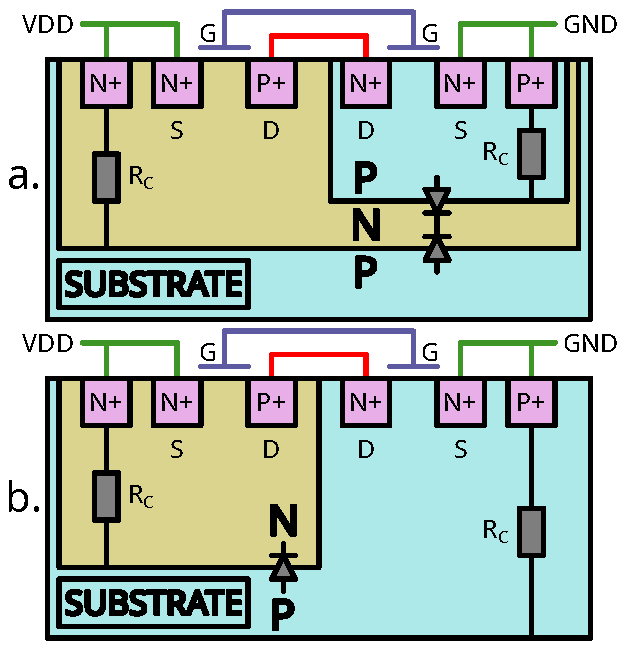
\includegraphics[width=0.35\textwidth]{./figures/substrate_2.pdf}
	\caption{Triple-well (a) and Dual-well (b) inverter cross-sectional view.}
	\label{fig_sub}
\end{figure}

		Because BBI can be performed thanks to the silicon substrate as the main physical environment transferring energy from a generator to an IC, it is fundamental to elaborate a proper substrate model to precisely represent the various involved phenomena.
		As stated previously, our work focuses on bulk substrates, and in most cases, the substrate silicon is P-doped.
		There are two typical ways of lithographing the transistors in a bulk substrate, using dual-well or triple-well structures.
		Dual-well substrates are commonly found in moderately old circuits, while triple-well substrates are found in more recent circuits, while not bleeding-edge.

		To properly understand how the differences between dual-well and triple-well substrates change the resulting model, let us analyze the cross-sectional schematics of an inverter created respectively in a triple-well and a dual-well substrate, as shown respectively in Fig. \ref{fig_sub}.a and Fig. \ref{fig_sub}.b:
		\begin{itemize}
			\item In the triple-well substrate, the NMOS transistors are lithographed into a P-doped silicon well, itself lithographed inside a N-doped well, buried inside the P-doped substrate. The PMOS transistors are located inside the N-doped well;
			\item In the dual-well substrate, the PMOS transistors are still located inside the N-doped well, however, the NMOS are lithographed directly inside the P-doped substrate.
		\end{itemize}
		On the one hand, the triple-well substrate reveals two diodes:
		\begin{itemize}
			\item One formed between the P-well and the N-well;
			\item Another formed between the N-well and the P-substrate.
		\end{itemize}
		On the other hand, the dual-well substrate only reveals one diode between the N-well and the P-substrate.

	\subsubsection{The resulting model}
		Thanks to what we have introduced previously, we can now build the elementary building blocks for our hybrid simulation flow.
		It combines the power delivery network architecture, the equivalent logic gates models, and the substrate structure, all in an embedded model.
		This model represents an elementary section of the simulated IC, measuring 30 \textmu m by 5 \textmu m by $t_{Sub}$ \textmu m, the latter being the substrate thickness, a parameter which will vary depending on each considered IC.
		% !TeX spellcheck = en_US
% !TeX root = ./0_article.tex

\begin{figure*}[ht]
	\centering
	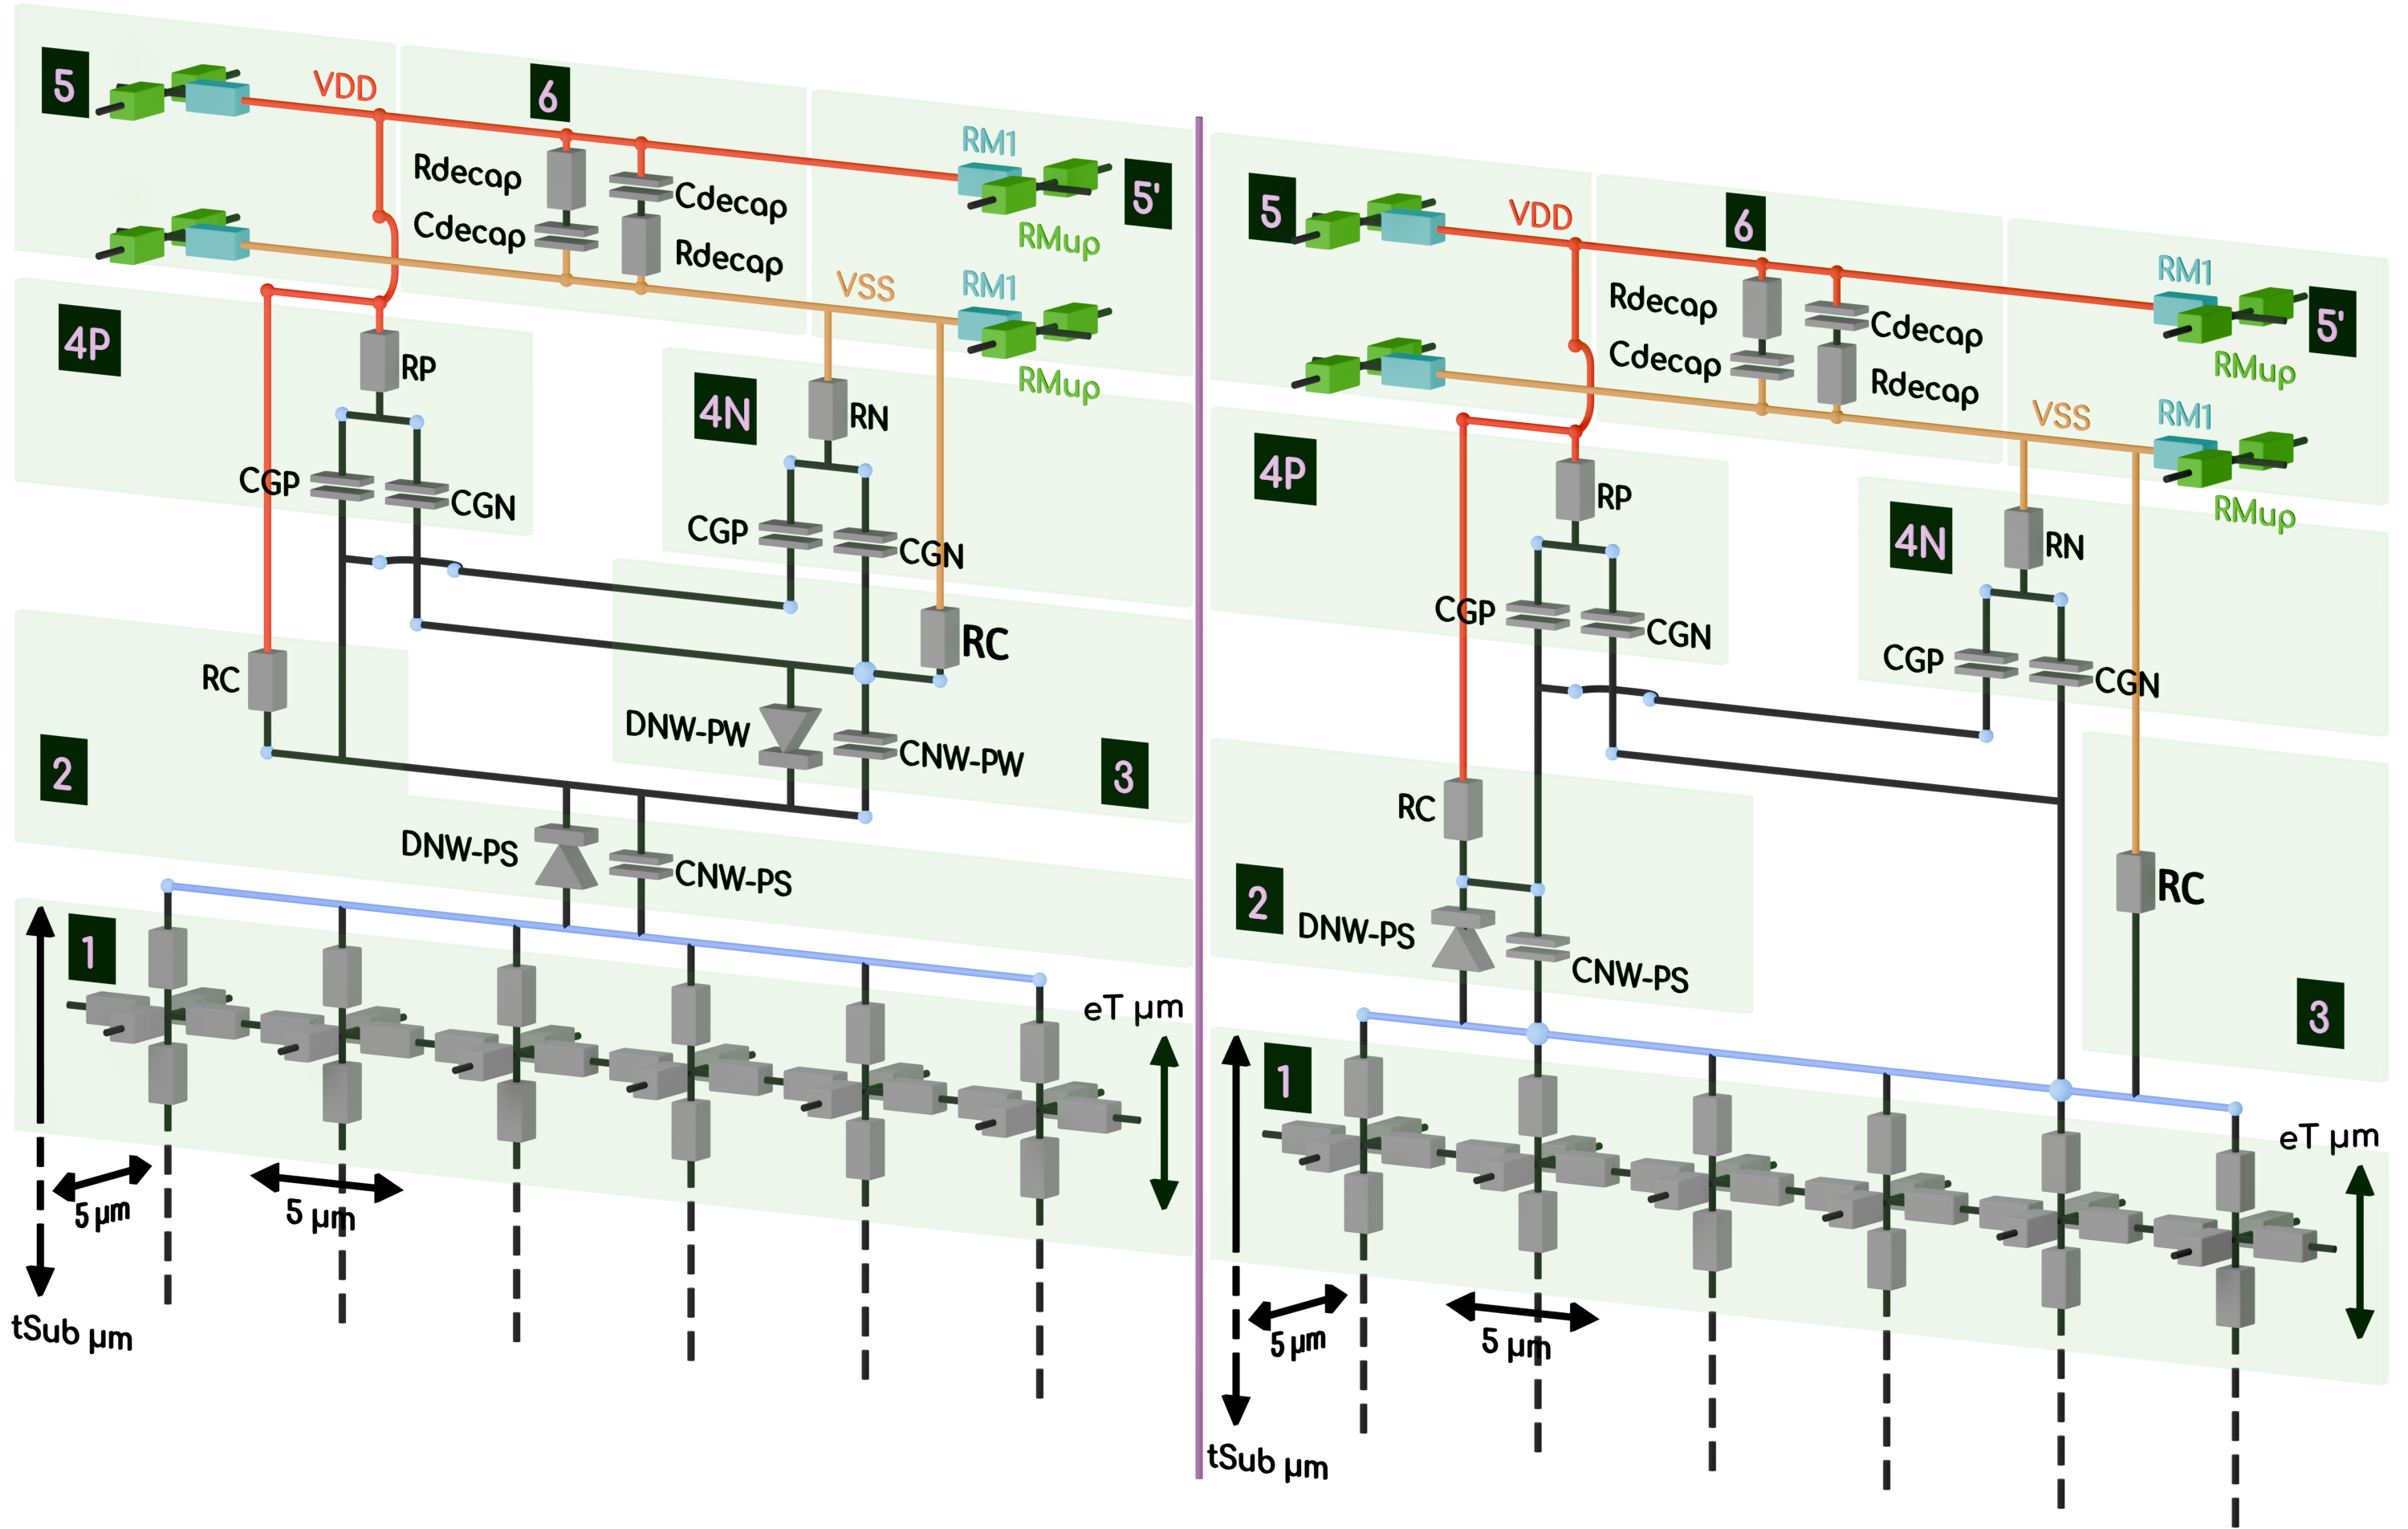
\includegraphics[width=0.95\textwidth]{./figures/dual+triple3.png}
	\caption{Triple well (left) and dual well (right) std cell \textcolor{red}{(PEUT ETRE FAIRE DES SOUS-FIGURES)}}
	\label{fig_triplewellstdcell}
\end{figure*}

		As we consider both triple-well and dual-well substrate, there are two resulting elementary models, shown in Fig. \ref{fig_triplewellstdcell}.
		Each model is composed of various sub-regions, whose descriptions follow:
		\begin{itemize}
			\item \ovalbox{1} is the substrate network, divided into six sub-networks of six resistors for finer details;
			\item \ovalbox{2} is the first P-N silicon junction, common to both models;
			\item \ovalbox{3} is the access resistor (DW) or the second junction (TW);
			\item \ovalbox{4P} is the PMOS equivalent section;
			\item \ovalbox{4N} is the NMOS equivalent section;
			\item \ovalbox{5, 5'} are the power supply metal layers (upper metal in green, first level in blue);
			\item \ovalbox{6} is the power supply decoupling.
		\end{itemize}
		As we have stated before, these models only represent a small portion of the modeled IC.
		To create an entire IC of a defined size, it is required to instantiate and interconnect as much as needed the elementary models.
		By doing so, we can create a bigger model of virtually any size.
		The language we have chosen to work with the simulation is the SPICE language.
		However, we created a custom Python script to interconnect the SCS together and generate a generic SPICE file.

\subsection{An hybrid simulation flow: performing simulations}
	Now that we set up the base models and their duplication, we can perform simulations with those models.
	To properly use these models, it is required, in the first place, to validate them through various steps to ensure their reliability.
	To that end, we generated an IC measuring 600 \textmu m by 600 \textmu m with a 200 \textmu m substrate thickness, and performed an operating point to verify the correctness of the models.
	% !TeX spellcheck = en_US
% !TeX root = ./0_article.tex

\begin{table}[H]
	\label{tab_op}
	\centering
	\begin{tabular}{lll}
		Value  & Triple-well & Dual-well \\ \hline
		$I_{GND}$                               & 2 nA          & 2.2 nA    \\
		$I_{VDD}$                                & -7 nA        & 3 nA        \\
		$\overline{GND_{drop}}$    & 2 nV         & 2 nV        \\
		$\overline{V_{DD_{drop}}}$    & 3 nV         & 3 nV       
	\end{tabular}
	\caption{op point}
\end{table}

%	% !TeX spellcheck = en_US
% !TeX root = ./0_article.tex

\section{Body biasing injection platforms modeling}
\IEEEPARstart{T}{he} objective of this first section is to present the work done concerning electrical modeling of integrated circuits in a BBI context.
Developing IC models in that specific case is not an easy task.
Indeed, modern digital ICs contains billions of transistors, and even considering microcontrollers where the transistor count is less important, with current technologies, it is impossible to evaluate circuits at a transistor level.

	\subsection{The hybrid simulation flow: introduction}
	To tackle these limitations, we decided to adopt an hybrid approach, combining transistor-less models and local logic gates simulations.
	This approach is a compromise between accuracy and computational cost/time, and allows simulating relatively big circuits under BBI disturbances.
	
	The resulting simulation flow is divided in three consecutive steps:
	\begin{itemize}
		\item The simulation of an IC under BBI using a transistor-less model, allowing for a purely electrical analysis;
		\item The extraction of significant disturbed signals from the previous simulation;
		\item The simulation of functional logic gates under BBI thanks to the previously extracted signals.
	\end{itemize}
	The first step allows analyzing IC macro-electrical behavior when subject to BBI, and at a lower computational cost compared to a functional model including transistors and internal transmission lines, even if it could be done in a reasonable time constraint for millions of transistors.
	Then, by extracting useful signals such as the power delivery and the transistor substrate voltages, we can evaluate what would be the behavior of actual logic gates subject to BBI.
	
	\subsection{The hybrid simulation flow : building the models}
	Building these models requires a correct understanding on integrated circuits internal structures, such as:
	\begin{itemize}
		\item The power supply network, composed of various stacked metal wires;
		\item The standard-cells, made of logic gates, and thus transistors, being pre-characterized cells used as building blocks;
		\item The silicon substrate, which can be of various type depending on the technology.
	\end{itemize}
	
		\subsubsection{Power supply rails and standard-cell segments}
		% !TeX spellcheck = en_US
% !TeX root = ./0_article.tex
% LABEL AFTER CAPTION WESH GEOFFREY !!
\begin{figure}[h]
	\centering
	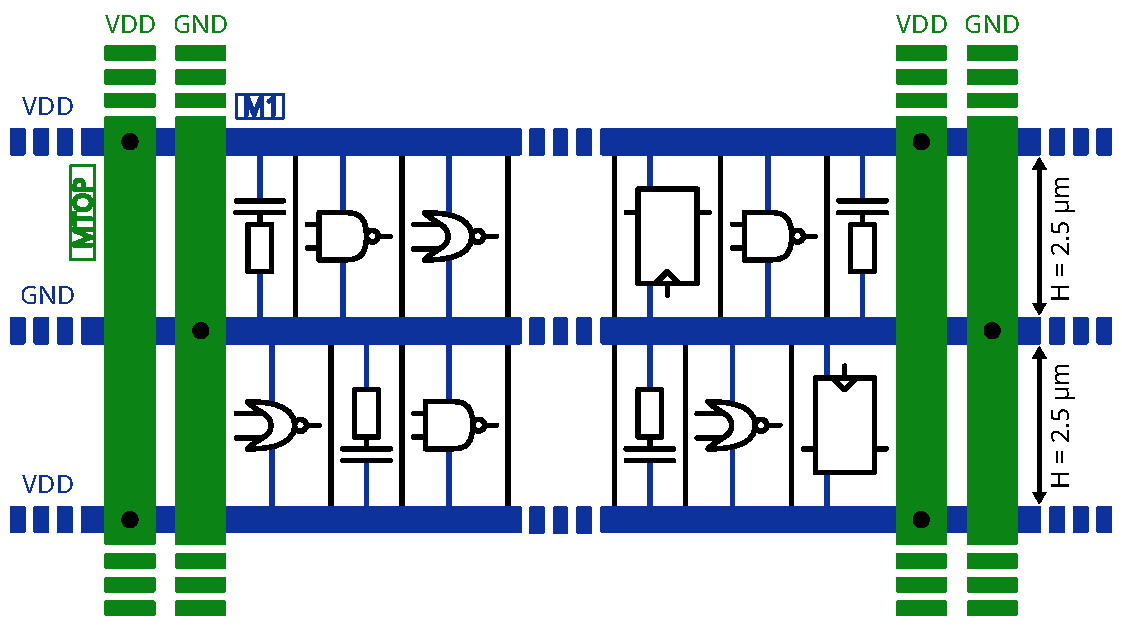
\includegraphics[width=0.49\textwidth]{./figures/psu_std_cell.pdf}
	\caption{A Standard-Cell Segment and its power delivery network.}
	\label{fig_alim_std}
\end{figure}

		The power distribution inside an IC is typically made with a grid-like structure, composed of metal wires stacked on top of each other on planes.
		The uppermost layer forms a ring surrounding the core.
		In each layer, the metal wires are equally spaced and have a dedicated width, which becomes thinner the deeper they are.
		The lowest layer brings the power directly to the transistors.
		
		Within these metal lines are located standard-cell segments (SCS), created by the power planning, as illustrated in Fig. \ref{fig_alim_std}.
		SCS are pre-characterized by foundries and classified according to their performance in timing and power consumption.
		Their height is fixed, while their width vary depending on their complexity, and are commonly made of logic gates, sequential, and decoupling elements.
	
		\subsubsection{Silicon substrate structure}
		Another important element of an IC is the substrate, and most importantly its type.
		We can mainly distinguish bulk and FD-SOI substrates.
		
		On the one hand, in bulk substrates, the transistor channel forms directly inside the P-substrate, and the depletion layer thickness is difficult to control.
		On the other hand, in FD-SOI substrates, a silicon oxide layer is created between the channel and the P-substrate, thus constraining the channel thickness.
		
		In this paper, we are focusing only on bulk substrates, and in this family, we can distinguish two substrate types: dual-well (DW) and triple-well (TW).
		The main difference between DW and TW substrates lies in how are lithographed NMOS transistors.
		In DW substrates, NMOS are located directly inside the P-doped substrate, and PMOS inside a N-doped well, called the N-well.
		However, in the case of a TW substrate, the PMOS are still inside the N-well, but the NMOS are located inside an additional P-doped well, made inside the N-well.
		
		These manufacturing differences are illustrated in Fig. \ref{fig_sub}, representing the cross-sectional view of an inverter made with a bulk technology.
		The PN and NP diodes formed between the substrate and the wells are represented, and the electrical resistances $R_C$ represent the access resistance of the substrate and the wells.
		% !TeX spellcheck = en_US
% !TeX root = ./0_article.tex

\begin{figure}[h]
	\centering
	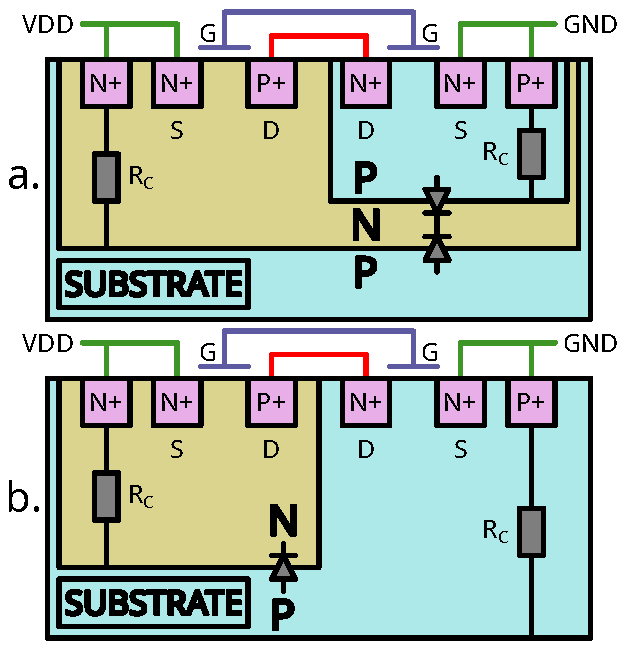
\includegraphics[width=0.35\textwidth]{./figures/substrate_2.pdf}
	\caption{Triple-well (a) and Dual-well (b) inverter cross-sectional view.}
	\label{fig_sub}
\end{figure}

		Dual-well substrates are found in moderately old ICs, while triple-well ones are common in more recent ICs, often coupled with dual-well substrate on the same die.
		The combination of both allows for \textcolor{orange}{cross-coupling noise reduction}, in addition to electrical insulation between transistors located on different domains (DW and TW).

		\subsubsection{Designing an elementary building-block for mass simulation}
		Thanks to the previously analyzed elements and models, we can now design elementary standard-cell blocks composed of the power delivery, the logic gates and the substrate, for each substrate type.
		As it has been said before, we are developing an hybrid simulation flow, therefore the designed elementary block is transistor-less.
		Eventually, our work is based on previous works on the subject \textcolor{cyan}{mathieuEMFI, FDTC2022, FDTC2023}.
		
		% !TeX spellcheck = en_US
% !TeX root = ./0_article.tex

\begin{figure*}[ht]
	\centering
	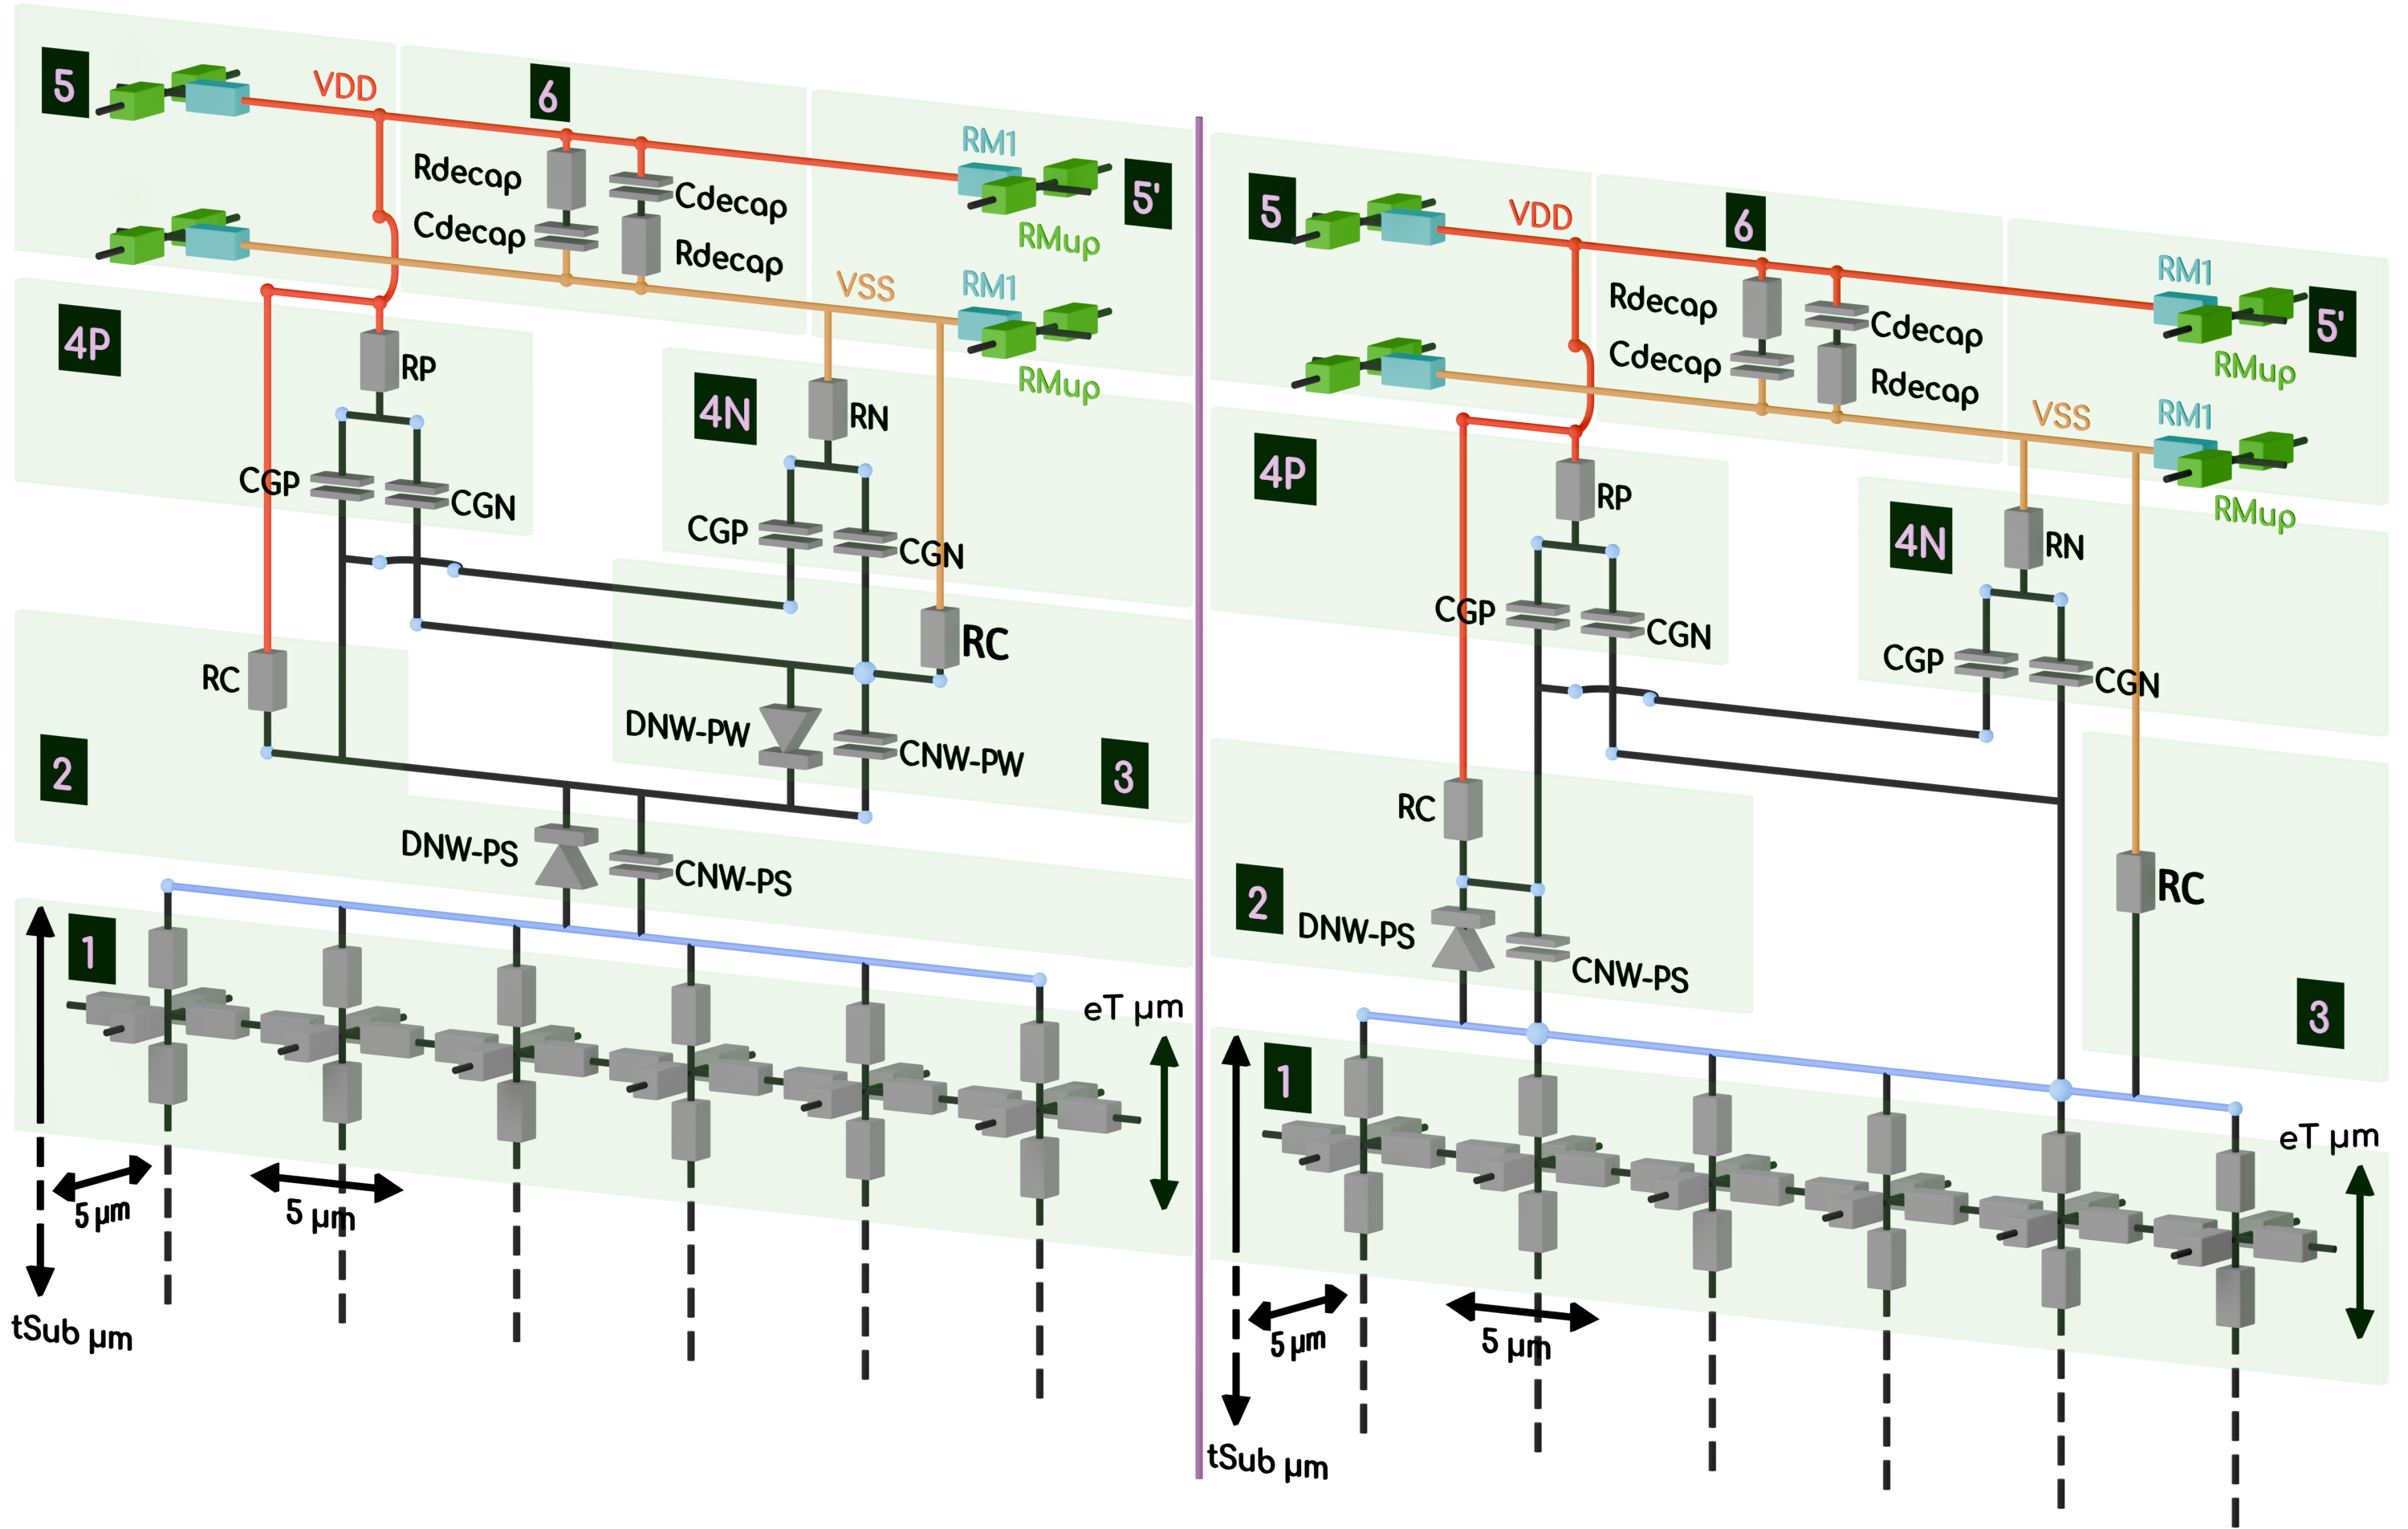
\includegraphics[width=0.95\textwidth]{./figures/dual+triple3.png}
	\caption{Triple well (left) and dual well (right) std cell \textcolor{red}{(PEUT ETRE FAIRE DES SOUS-FIGURES)}}
	\label{fig_triplewellstdcell}
\end{figure*}

		
		The model we propose is shown in Fig. \ref{fig_triplewellstdcell} both for a triple-well and a dual-well substrate.
		The models are extremely similar, but their difference is what is important.
		It represents an entire standard-cell segment, including a two levels power delivery network, average models of a hundred of logic gates, silicon junctions, and the silicon substrate.
		For better clarity, we divided the model into 6 sections, each representing a specific building block:
		\begin{itemize}
			\item \shadowbox{1} The substrate: modeled with 6 blocks of 6 resistors;
			\item \shadowbox{2} The P-N substrate-well silicon junction;
			\item \shadowbox{3} The N-P well-well silicon junction (TW), or the substrate access resistance (DW);
			\item \shadowbox{4N} \shadowbox{4P} The MOS average electrical model;
			\item \shadowbox{5} \shadowbox{5'} The power distribution metals;
			\item \shadowbox{6} The power supply decoupling.
		\end{itemize}
		The component values are calculated according to the target technology, in our case 90 nm, and are shown in Table \ref{tab_scs_numeric}

%\subsection{The hybrid simulation flow : building the models}
%The transistor-less model, also called standard-cell model, is developed thanks to the internal structure of integrated circuits, including:
%\begin{itemize}
%	\item Their power supply network;
%	\item Their standard-cells properties;
%	\item Their silicon substrate.
%\end{itemize}
%These three elements and their internal structure allow elaborating average models, able to represent their macro behavior.
%Fig. \ref{fig_alim_std} illustrates the base symbolic diagram used for our design.
%It represents a standard-cell segment, composed of logic gates and decoupling elements, with a fixed height of 5 µm and a variable width.
%For simplicity, two levels of metals for the power distribution are represented, the highest level MTOP in green and the first level M1 in blue.
%
%Then, because the previous analysis does not consider the substrate on which the transistors lie, it is required to extend the model.
%To that end, we represent in Fig. \ref{fig_sub} the cross-sectional view of a CMOS inverter in a triple-well and dual-well substrate.
%The parasitic silicon diodes formed between the substrate and the N-well, and between the N-well and the P-well are represented, in addition to the wells access electrical resistances $R_C$.
%
%Thanks to these preliminary analysis and former work on the subject \textcolor{cyan}{mathieuEMFI, fdtc20222023}, we set up an elementary transistor-less model, considering every presented aspect.
%This model, shown in Fig. \ref{fig_triplewellstdcell} for a triple-well substrate, represents a column portion of an IC, being 30 µm wide, 5 µm deep, and tSub µm thick.
%The schematic is divided into 6 sections:
%\begin{itemize}
%	\item \shadowbox{1} The substrate model, an array of distributed resistors;
%	\item \shadowbox{2} The P-N substrate-well silicon junction;
%	\item \shadowbox{3} The N-P well-well silicon junction;
%	\item \shadowbox{4N} \shadowbox{4P} The MOS average electrical model;
%	\item \shadowbox{5} \shadowbox{5'} The power distribution metals;
%	\item \shadowbox{6} The power supply decoupling.
%\end{itemize}
%The passive components modeling the transistors represent about 100 hundreds logic gates in the target technology.
%Therefore, the model allows evaluating simultaneously the average electrical behavior of 100 hundreds logic gates at a very low cost.
%
%% !TeX spellcheck = en_US
% !TeX root = ./0_article.tex
% LABEL AFTER CAPTION WESH GEOFFREY !!
\begin{figure}[h]
	\centering
	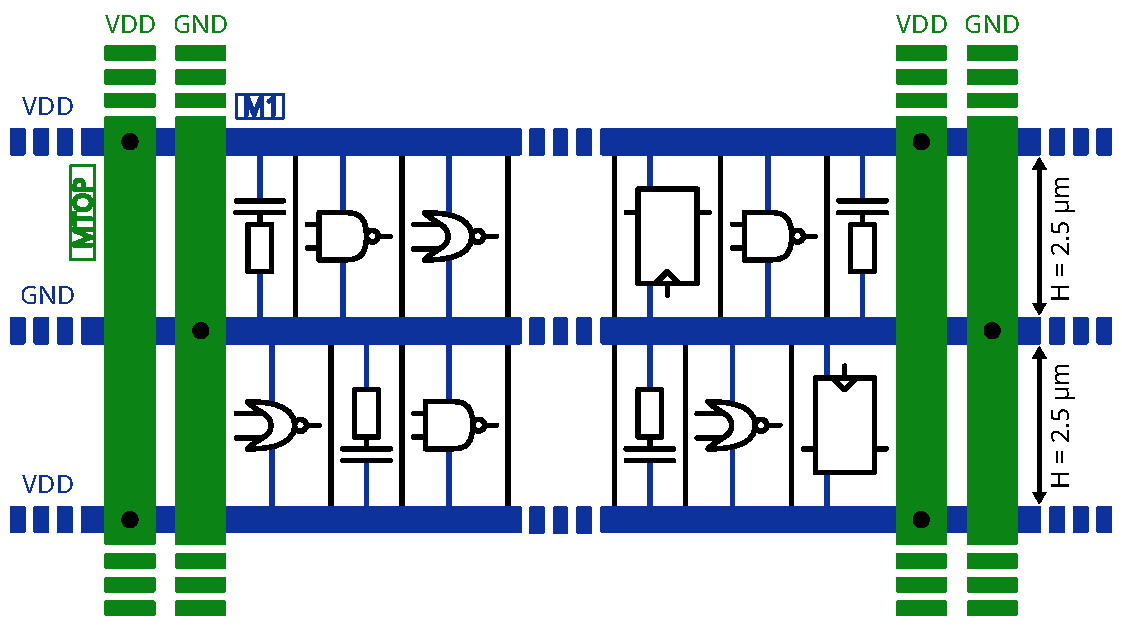
\includegraphics[width=0.49\textwidth]{./figures/psu_std_cell.pdf}
	\caption{A Standard-Cell Segment and its power delivery network.}
	\label{fig_alim_std}
\end{figure}

%
%% !TeX spellcheck = en_US
% !TeX root = ./0_article.tex

\begin{figure}[h]
	\centering
	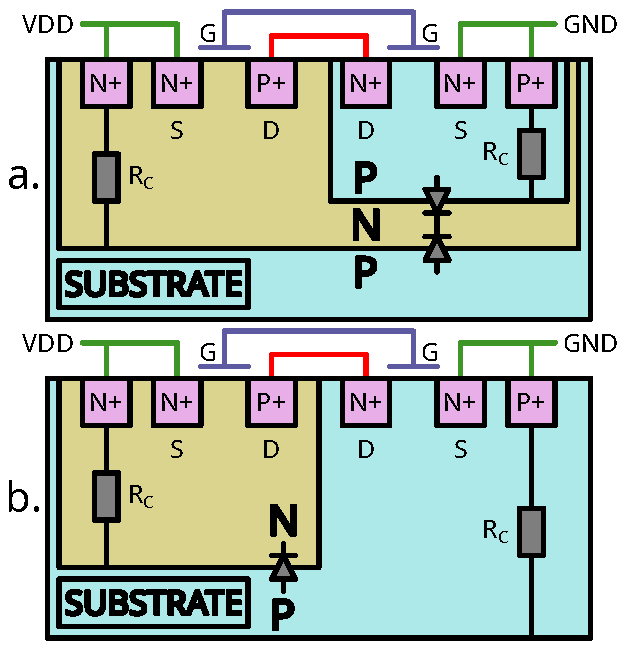
\includegraphics[width=0.35\textwidth]{./figures/substrate_2.pdf}
	\caption{Triple-well (a) and Dual-well (b) inverter cross-sectional view.}
	\label{fig_sub}
\end{figure}

%
%% !TeX spellcheck = en_US
% !TeX root = ./0_article.tex

\begin{figure*}[ht]
	\centering
	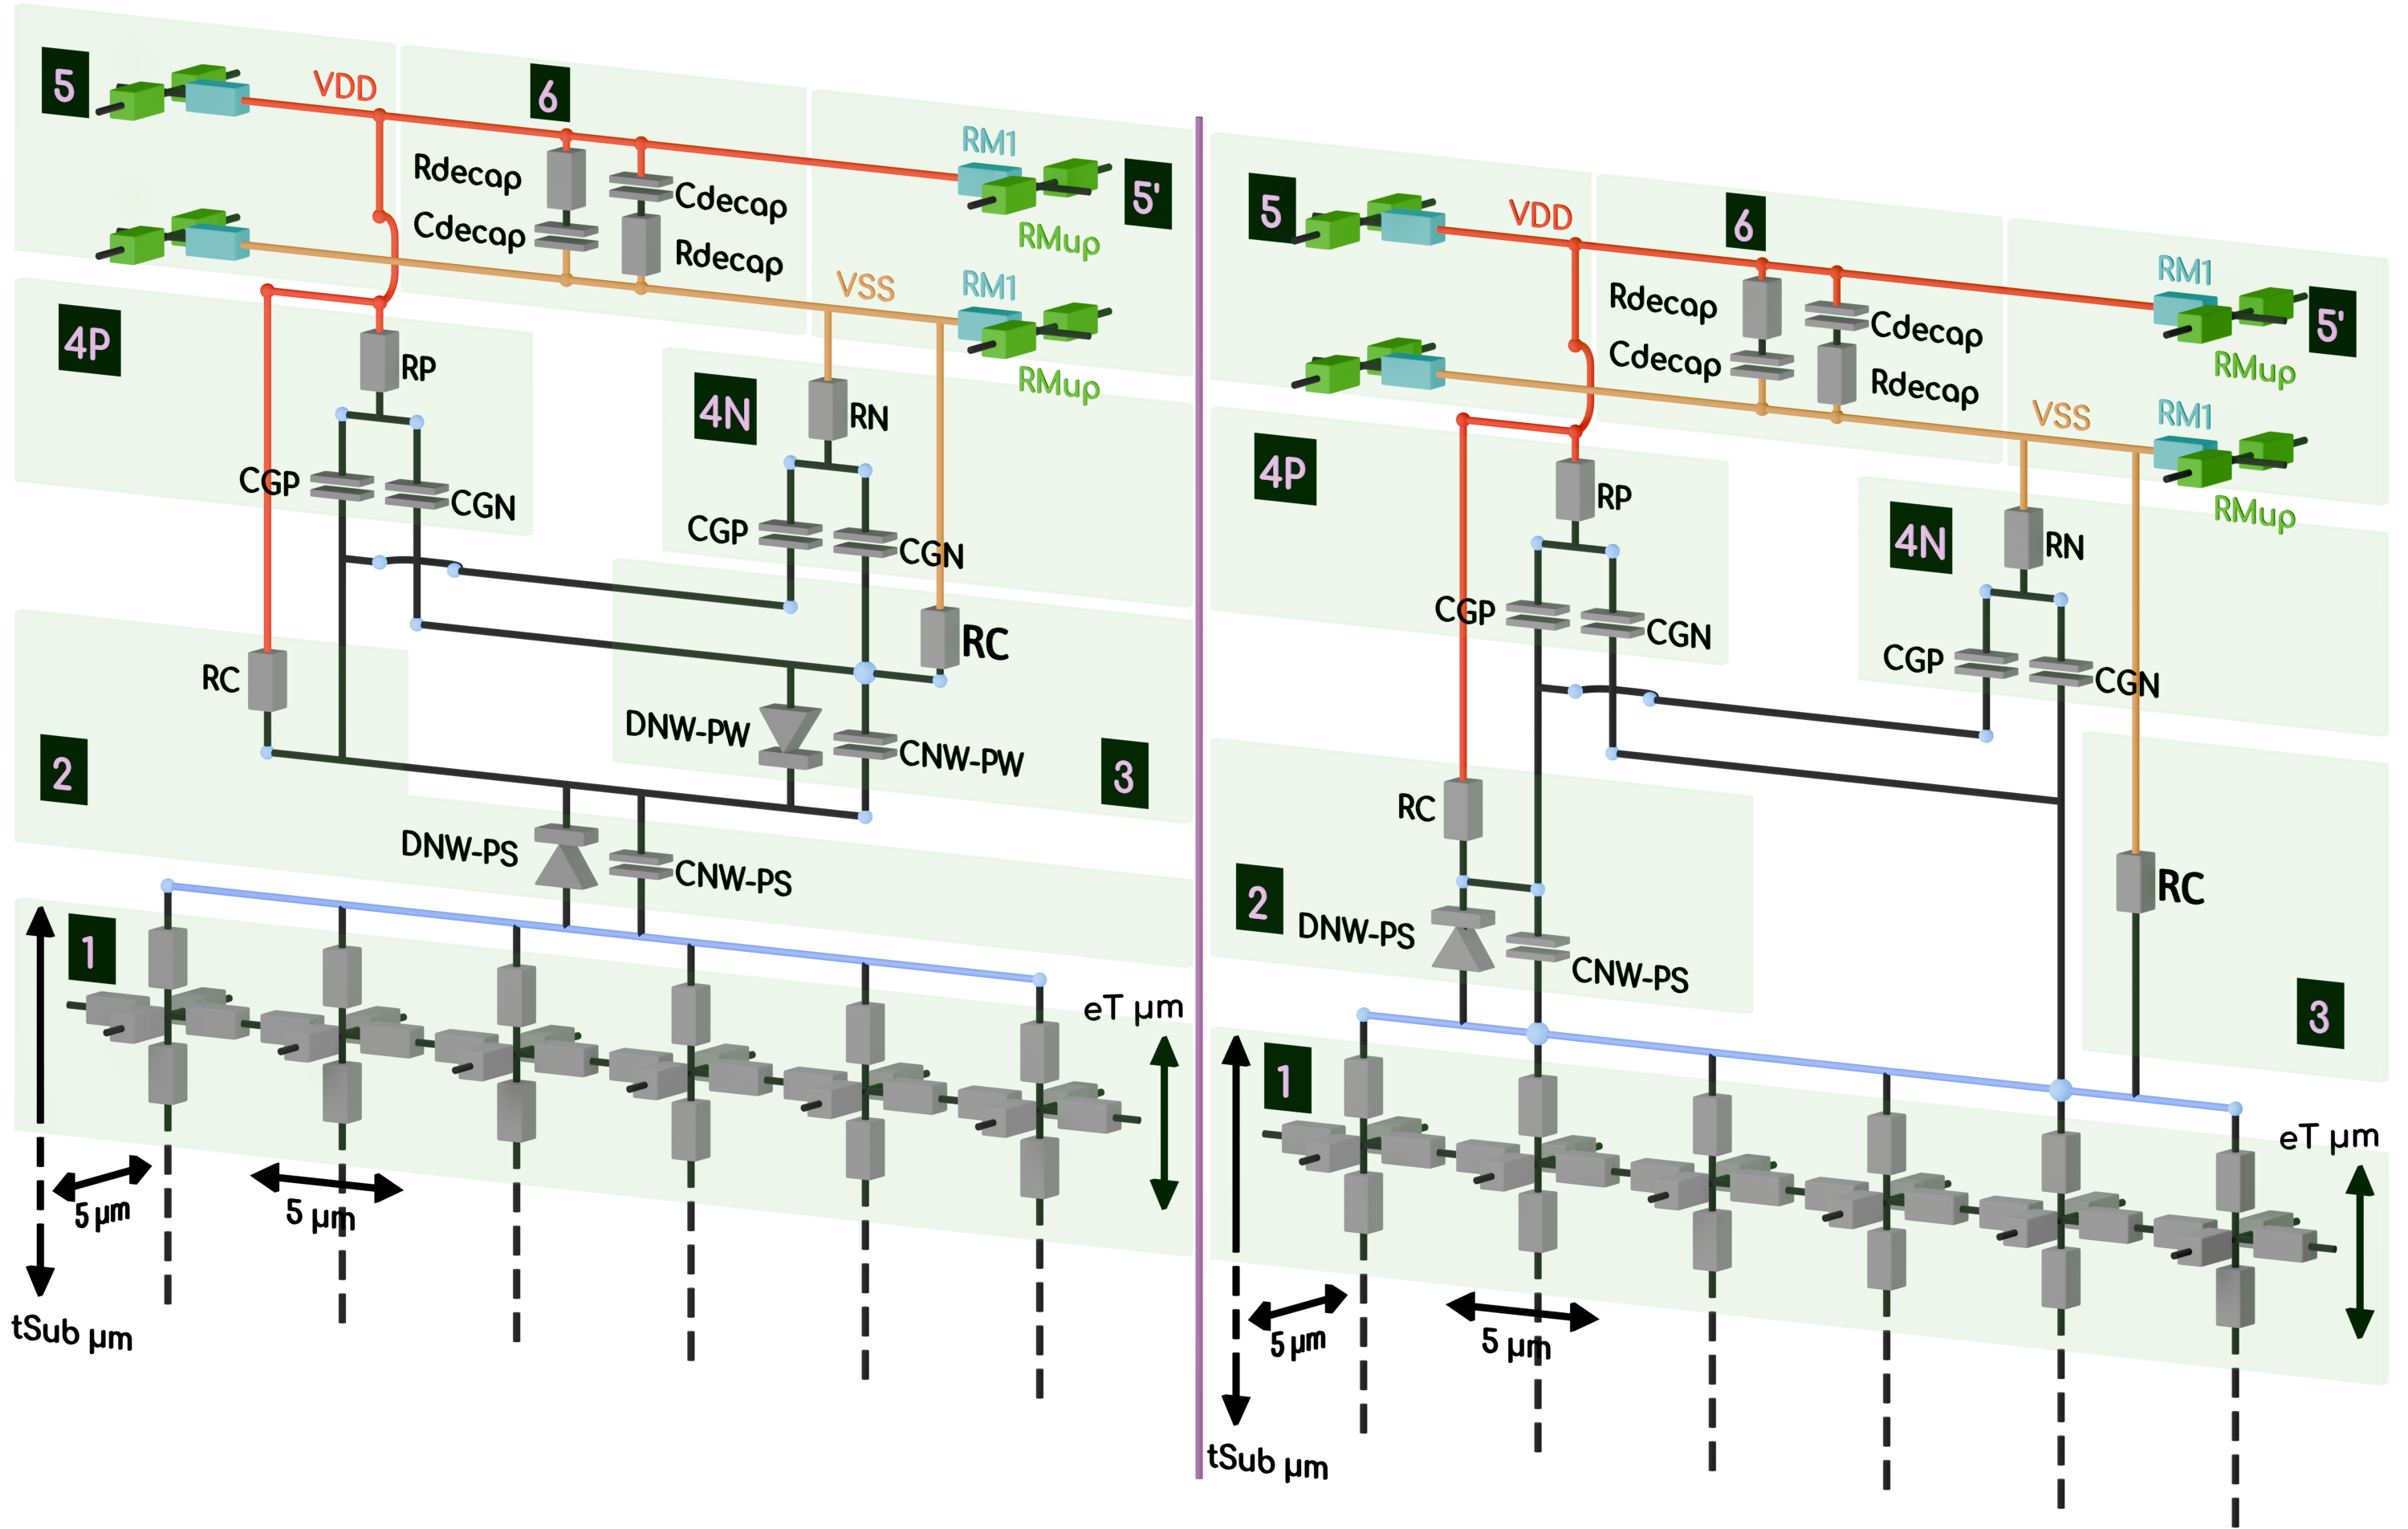
\includegraphics[width=0.95\textwidth]{./figures/dual+triple3.png}
	\caption{Triple well (left) and dual well (right) std cell \textcolor{red}{(PEUT ETRE FAIRE DES SOUS-FIGURES)}}
	\label{fig_triplewellstdcell}
\end{figure*}


%	% !TeX spellcheck = en_US
% !TeX root = ./0_article.tex

\section{Hybrid simulation results}

%	% !TeX root = ./0_article.tex

\section{Logic path under BBI}
For the purpose of analyzing the effects og BBI on actual logic, this section is dedicated in modeling and simulating an actual logic path
In this section, we are lingering on analyzing the effects of BBI on more complex logic paths.
The study is conducted for both a static logic path and a dynamic logic path.
The considered logic paths are constituted of inverters, buffers and a D-Flip-Flop (DFF).
The inverters model an arbitrary combinatorial logic path tackling the input of a DFF, used to sample the logic path output.
The DFF clock is buffered to achieve an isolation from the ideal voltage source.
Then, the DFF output is injected into a final 4-IVX chain, loaded with a 5 pF capacitor.
The resulting schematic is described in Fig. \ref{dffChain}.

\begin{figure}[h]
	\label{dffChain}
	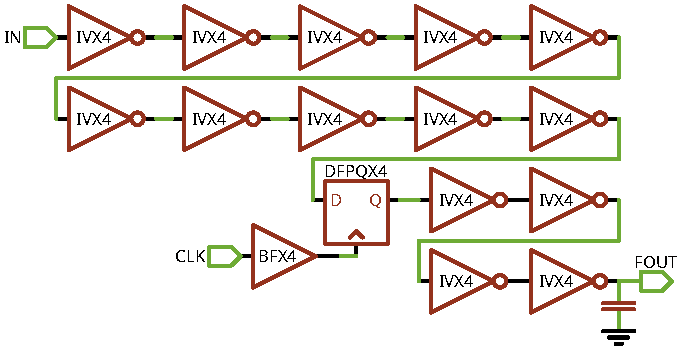
\includegraphics[width=0.5\textwidth]{./figures/dff_ivx_chain_2.pdf}
	\caption{DFFCHAIN}
\end{figure}

%	% !TeX root = ./0_article.tex

\section{Body biasing injection platforms overhaul}
\IEEEPARstart{T}{his} second section is dedicated in analyzing the various improvements we set up to enhance BBI reproducibility.
In the first place, we are going to analyze the various platforms proposed in the state-of-the art, then confront them to the proposed platform.
%	% !TeX spellcheck = en_US
% !TeX root = ./0_article.tex

\section{Conclusion}
	\IEEEPARstart{B}{ody} biasing injection has seen a re-emergence since 2020 \cite{bbiColin}, and various works have brought more and more knowledge throughout the years.
	BBI, contrary to EMFI or LFI, uses the silicon substrate of as the main physical medium to interact, transfer energy, and disturb integrated circuits.
	We introduced, through this work, the cumulative knowledge we gathered concerning BBI.
	This involves various aspects of the subjects.

	First, we studied better methods to improve BBI experiments repeatability and reliability through low-cost platform modifications.
	We supported these results with actual experiments such as Fault Analysis Mappings and a Differential Fault Attack.

	Then, we introduced large-scale IC modeling thanks to the use of transistor-less models allowing to reduce the computational power required to simulate BBI.

	Eventually, we extended this "transistor-less models" simulation flow to consider the logic functions of integrated circuits under BBI.
	This allowed us to understand the mechanisms at work during fault creation in integrated circuits under BBI, such as data-dependent bit set/reset faults, in addition to understanding the locality of BBI effects.

%	\begin{thebibliography}{1}
	\bibliographystyle{unsrt}
	\bibliography{references.bib}
%	\end{thebibliography}

\end{document}
